\documentclass[../main.tex]{subfiles}
\begin{document}
\chapter{Higher Order Linear ODEs}
We will focus on 2nd order here, but many methods are also applicable to higher orders.
\section{Constant Coefficients}
The general form of a 2nd order linear ODE with constant coefficients is:
\begin{equation}
  \label{general2ndConst}
  \underbrace{a \deriv[2]{y}{x} + b \deriv{y}{x} + cy}_{\mathcal{D}y} = f(x)
\end{equation}
with $a, b, c$ constants.
Where $\mathcal{D}y$ is a linear differential operator, defined as:
\[
  \mathcal{D} \equiv a \deriv[2]{}{x} + b \deriv{}{x} + c
\]
\begin{definition}[Linear Operator]
  A differential operator, $\mathcal{D}$ is \textit{linear} if for any $y_1(x)$ and $y_2(x)$ and constants $\alpha$ and $\beta$:
  \[
    \mathcal{D}(\alpha y_1 + \beta y_2) = \alpha \mathcal{D}y_1 + \beta \mathcal{D}y_2
  \]
  This is also known as the \textit{principle of superposition}.
\end{definition}
We can exploit this property to solve \cref{general2ndConst}:
\label{constantCoeffMethod}
\begin{enumerate}
  \item Find complimentary functions (C.F.), $y_c$, that satisfy the corresponding homogeneous equation:
    \[
      a \deriv[2]{y_c}{x} + b \deriv{y_c}{x} + c y_c = 0
    \]
  \item Find \textbf{any} particular integral (P.I.), $y_p$ that satisfies the full equation.
  \item Then a solution of the full equation is then $y_c + y_p$ as:
    \[
      \mathcal{D}(y_c + y_p) = \underbrace{\mathcal{D}y_c}_{=0} + \mathcal{D}y_p = f(x)
    \]
    So it satisfies the full equation.
\end{enumerate}
A 2nd order ODE has \textbf{two} linearly independent complimentary functions, so the general solution to is:
\[
  y(x) = C_1 y_{c_1}(x) + C_2 y_{c_2}(x) + y_p(x)
\]
with $C_1, C_2$ constants.
\begin{definition}[Linear Dependance]
  A set of $n$ functions $\{f_i(x)\}$ is \textit{linearly dependant} if:
  \[
    \sum_{i=1}^{n} C_i f_i(x) = 0\ \forall x
  \]
  for $n$ constants, $C_i$, \textbf{not} all of which are $0$.
  Otherwise they are \textit{linearly independent}.
\end{definition}
\begin{remark}
  This is the same idea as linear dependence for vectors.
\end{remark}
Equivalently, if one or more of the functions $f_i(x)$  can be written as a linear combination of the others, they are linearly \textbf{dependant}.
\subsection{Complimentary Functions}
Recall that:
\[
  \deriv{}{x} e^{\lambda x} = \lambda e^{\lambda x} \text{ (Eigenfunction)}
\]
$e^{\lambda x}$ is also an eigenfunction of $\mathcal{D}$ because:
\begin{align*}
  \mathcal{D}(e^{\lambda x}) &= a \deriv[2]{}{x} e^{\lambda x} + b \deriv{}{x} e^{\lambda x} + c \\
                             &= \underbrace{(a\lambda^2 + b\lambda + c)}_{\text{eigenvalue}} e^{\lambda x}
\end{align*}
The complimentary functions of \cref{general2ndConst} satisfy $\mathcal{D}y_c = 0$, that is, they are eigenfunctions with eigenvalue $0$.
Thus:
\[
  y_c = A e^{\lambda x} \text{ with } \underbrace{a \lambda^2 + b\lambda + c = 0}_{\text{characteristic equation}}
\]
Since the characteristic equation of $\mathcal{D}$ is a 2nd degree polynomial it must have two roots $\lambda_1$ and $\lambda_2$.
\begin{proofcases}
  \begin{case}{$\lambda_1 \neq \lambda_2$}
    We then have two linearly independent complimentary functions:
    \[
      y_{c_1} \propto e^{\lambda_1 x}, y_{c_2} \propto e^{\lambda_2 x}
    \]
    So the most general complimentary function is a linear combination:
    \[
      y_c = C_1 y_{c_1}(x) + C_2 y_{c_2}(x)
    \]
    So $y_{c_1}$ and $y_{c_2}$ for a \textit{basis} for the space of solutions for the homogeneous equation.
    Note that if the roots are complex, we get oscillatory behaviour.

    \begin{remark}
      If the roots of the characteristic equation are $\pm k \in \R$, it is often advisable to use the general form:
      \[
        y_c = A\cosh kx + B \sinh kx
      \]
    \end{remark}
  \end{case}
  \begin{case}{$\lambda = \lambda_2$ -- Degenerate Case}
    So now we have only one linearly independent complimentary function of the form $e^{\lambda_1 x}$.
    See \cref{detuningExample} for how to deal with this case.
  \end{case}
\end{proofcases}
\begin{example}[Real, non-degenerate roots]
  \[
    \deriv[2]{y}{x} - 5\deriv{y}{x} + 6y = 0
  \]
  The characteristic equation is then:
  \[
    \lambda^2 - 5\lambda + 6 = 0 \implies \lambda_1 = 3, \lambda_2 = 2
  \]
  So the general complimentary function is:
  \[
    y_c(x) = A e^{3x} + B e^{2x}
  \]
  with $A, B$ constants.
\end{example}
\begin{example}[Complex, non-degenerate roots]
  \label{complexNonDegenerate}
  \[
    \deriv[2]{y}{x} + 4y = 0
  \]
  The characteristic equation is then:
  \[
    \lambda^2 + 4 = 0 \implies \lambda_1 = 2i, \lambda_2 = -2i
  \]
  So the general complimentary function is:
  \[
    y_c(x) = Ae^{2ix} + Be^{-2ix}
  \]
  Note that $e^{\pm2ix} = \cos(2x) \pm i \sin(2x)$ so:
  \begin{align*}
    y_c(x) &= (A + B)\cos(2x) + (A - B)i\sin(2x) \\
           &= \alpha \cos(2x) + \beta \sin(2x)
  \end{align*}
  Whether $\alpha, \beta$ are complex depends on the boundary conditions of the problem.
\end{example}
\begin{example}[Degenerate roots and ``detuning'']
  \label{detuningExample}
  \[
    \deriv[2]{y}{x} - 4\deriv{y}{x} + 4y = 0
  \]
  So the characteristic equation is:
  \[
    \lambda^2 - 4y + 4 = 0 \implies \lambda = 2
  \]
  Therefore we have degenerate roots and only one linearly independent complimentary function $e^{2x}$.

  \textbf{Detuning - }Remove the degeneracy by considering a slightly modified (\textit{detuned}) equation.
  \[
    \deriv[2]{y}{x} - 4 \deriv{y}{x} + (4 - \varepsilon^2)y = 0 \quad (\varepsilon \ll 1)
  \]
  So the characteristic equation is now:
  \[
    \lambda^2 - 4\lambda + (4 - \varepsilon^2) = 0 \implies \lambda = 2 \pm \varepsilon
  \]
  Which gives the complimentary function:
  \begin{align*}
    y_c(x) &= Ae^{(2 + \varepsilon)x} + Be^{(2 - \varepsilon)x} \\
           &=e^{2x}(Ae^{\varepsilon x} + Be^{-\varepsilon x}) \\
           &=e^{2x}[(A+B) + \varepsilon(A - B)x + O(A\varepsilon^2x^2) + O(B\varepsilon^2x^2)] \text{ (as $\varepsilon \to 0$)} \\
  \end{align*}
  Apply the initial conditions $y(0) = C$ and $y'(0) = D$ to both the original and detuned equations.
  This yields the equations:
  \begin{align*}
    &A + B = C \text{ and } 2C + \varepsilon(A - B) = D \\
    \implies& A = \frac{1}{2}\left(C + \frac{D - 2C}{\varepsilon}\right),\ B = \frac{1}{2}\left(C - \frac{D - 2C}{\varepsilon}\right)
  \end{align*}
  So $O(A) \text{ and } O(B) = O(\frac{1}{\varepsilon})$ as $\varepsilon \to 0$.
  Therefore $O(A\varepsilon^2x^2) \text{ and } O(B\varepsilon^2x^2) = O(\varepsilon x^2) \to 0$ as $\varepsilon \to0$.

  Now let:
  \[
    \alpha = A + B, \beta = \varepsilon(A - B)
  \]
  Both $\alpha$ and $\beta$ are $O(1)$ as they do not depend on $\varepsilon$ so are unchanged as $\varepsilon \to 0$.
  As we take $\varepsilon \to 0$, the detuned equation becomes the original equation, so the general solution of the original degenerate equation is:
  \[
    y = \alpha e^{2x} + \beta x e^{2x}
  \]
\end{example}
\begin{remark}[Note]
  In general, if $y_{c_1}$ is a degenerate complimentary function of a linear ODE with constant coefficients then $y_{c_2} = x y_{c_1}$ is a second linearly independent complimentary function.
\end{remark}
\section{Homogeneous Second Order ODEs with Non-constant Coefficients}
The general form of a homogeneous second order ODE with non-constant coefficients is:
\[
  y'' + p(x)y' + q(x)y = 0
\]
\subsection{Second Complimentary Function -- Reduction of order}
\label{reductionOrder}
The following method allows us to find a second solution, $y_2(x)$, given one solution, $y_1(x)$.

We try a solution of the form $y_2(x) = v(x)y_1(x)$.
Therefore:
\[
  y_2' = v'y_1 + vy_1' \text{ and } y_2'' = v''y_1 + 2v'y_1' + vy_1''
\]
If $y_2$ satisfies the original ODE then we require that:
\begin{align*}
  v''y_1 + v'(2y_1' + py_1) + v(\underbrace{y_1'' + py_1' + qy_1}_{0}) &= 0 \\
  v''y_1 + v'(2y_1' + py_1) &= 0
\end{align*}
We can then let $u = v'$ to reduce the order of the DE:
\[
  u'y_1 + u(2y_1' + py_1) = 0
\]
This is now a separable first order ODE for $u$.
\begin{align*}
  \frac{u'}{u} &= -\frac{2y_1'}{y_1} - p \\
  \implies \ln u &= -2 \ln y_1  - \int^{x} p(t) \d{t} + \ln A \\
  \implies u(x) &= \frac{A}{y^{2}_{1}}\exp\left[-\int^{x} p(t) \d{t}\right]
\end{align*}
We can then, in theory, integrate this expression for $u(x)$ to obtain $v(x)$.
\begin{example}
  Consider again the DE from \cref{detuningExample}:
  \[
    y'' - 4y' + 4y = 0
  \]
  So $p(x) = -4, q(x) = 4$.
  We know that one solution is $y_1(x) = e^{2x}$.
  \[
    \frac{u'}{u} = -\frac{4e^{2x}}{e^{2x}} - (-4) = 0
  \]
  So $u$ and therefore $v'$ are constants so:
  \[
    v(x) = Ax+B
  \]
  Therefore we have a second solution $y_2$ given by:
  \[
    y_2(x) = (Ax + B)e^{2x}
  \]
  The $Be^{2x}$ replicates $y_1$ so $xe^{2x}$ is a second linearly independent solution.
\end{example}
\subsection{Phase Space}
\label{phaseSpaceSec}
The general form of an $n$-th order linear ODE is:
\[
  y^{(n)} + p_1(x)y^{(n-1)} + \cdots + p_n(x)y = f(x)
\]
This means that $y^{(n)}$ is determined by $y^{(0)}, \ldots, y^{(n-1)}$.
When we differentiate the equation, we see that higher order derivatives can also be determined by $y^{(0)}, \ldots, y^{(n-1)}$.
This means that we can construct a Taylor series about $x_0$ if we specify $y^{(0)}(x_0), \ldots, y^{(n-1)}(x_0)$.

In other words, the \textit{state of the system} is fully specified at any $x$ by an $n$-dimensional \textit{solution vector}:
\[
  \vec{Y}(x) = \begin{pmatrix}
  y(x) \\
  y^{(1)}(x) \\
  \vdots \\
  y^{(n-1)}(x) \\
  \end{pmatrix}
\]
That is, given such a $\vec{Y}(x_0)$ at any fixed $x_0$, we can determine the Taylor series for the solution and use this to determine $y$ and all of its derivatives at any $x$.
\begin{remark}
  \begin{itemize}
    \item At any $x$, $\vec{Y}(x)$ defines a point in $n$-dimensional \textit{phase space}.
    \item As $x$ varies, $\vec{Y}(x)$ traces a trajectory through \textit{phase space}.
  \end{itemize}
\end{remark}
\begin{example}
  Consider again the DE from \cref{complexNonDegenerate}:
  \[
    y'' + 4y = 0
  \]
  We know that $y_1(x) = \cos 2x$ and $y_2(x) = \sin 2x$ so the solution vectors are:
  \[
    \vec{Y}_1 = \begin{pmatrix}
    y_1 \\
    y_1' \\
    \end{pmatrix} =
    \begin{pmatrix}
    \cos 2x \\
    -2\sin 2x \\
    \end{pmatrix},\
    \vec{Y}_2 = \begin{pmatrix}
    y_2 \\
    y_2 \\
    \end{pmatrix} =
    \begin{pmatrix}
    \sin 2x \\
    2 \cos 2x \\
    \end{pmatrix}
  \]
  So in 2D phase space, $\vec{Y}_1$ and $\vec{Y}_2$ lie on the same ellipse:
  \begin{center}
  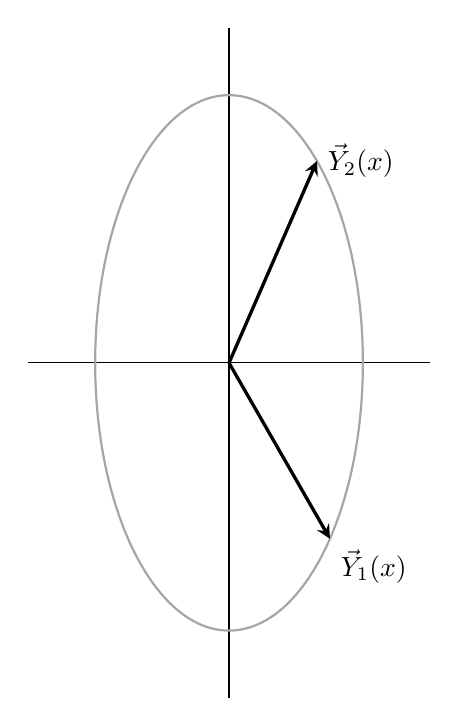
\begin{tikzpicture}[scale=1.7, >=stealth]
    \draw[-] (-1.5, 0) -- (1.5, 0);
    \draw[-] (0, -2.5) -- (0, 2.5);

    \draw[thick, gray!70] (0, 0) ellipse (1 and 2);

    \draw[->, very thick] (0, 0) -- (0.7539, -1.3139) node[below right] {$\vec{Y}_1(x)$};
    \draw[->, very thick] (0, 0) -- (0.6569, 1.5078) node[right] {$\vec{Y}_2(x)$};
  \end{tikzpicture}
  \end{center}
  $\vec{Y}_1$ and $\vec{Y}_2$ are linearly independent vectors.
  This means that they form a basis for the 2D phase space.
\end{example}
\section{Wronskian and Linear Dependence}
\label{wronskian}
Recall that a set of functions $\{y_i(x)\}$ are linearly dependant if:
\[
  \sum_{i=1}^{n} c_i y_i(x) = 0\ \forall x,\ c_i \text{ not all 0}
\]
Since this holds for all $x$ we can differentiate it $1, 2, \ldots, n-1$  times.
Therefore:
\[
  \sum_{i=1}^{n} c_i y^{(k)}_i(x) = 0\ \forall x, k = 1, \ldots, n-1
\]
This sum the $k$-th entry in the sum of all the solution vectors, so we have:
\[
  \sum_{i=1}^{n} c_i \vec{Y}_i(x) = 0\ \forall x
\]
So if $\{y_i\}$ is linearly dependant, then $\{\vec{Y}_i(x)\}$ are linearly dependant for all $x$.

We can form a \textit{fundamental matrix}, $\Psi(x)$, whose columns are the solution vectors:
\[
  \Psi(x) = \begin{pmatrix}
  \uparrow & \uparrow &  & \uparrow \\
  \vec{Y}_1 & \vec{Y}_2 & \cdots & \vec{Y}_n \\
  \downarrow & \downarrow &  & \downarrow \\
  \end{pmatrix}
\]
\begin{definition}[Wronskian]
  The \textit{Wronskian} of $n$ functions $\{y_i\}$ is defined to be the following determinant:
  \[
    W(x) =
    \begin{vmatrix}
      y_1 & y_2 & \cdots & y_n \\
      y_1' & y_2' & \cdots & y_n' \\
      \vdots & \vdots & \ddots & \vdots \\
      y^{(n-1)}_1 & y^{(n-1)}_2 & \cdots & y^{(n-1)}_n \\
    \end{vmatrix}
  \]
\end{definition}
\begin{remark}[Note]
  In this case, the Wronskian is the determinant of the fundamental matrix, that is:
  \[
    W(x) =
    \det(\Psi(x)) =
    \begin{vmatrix}
      \uparrow & \uparrow &  & \uparrow \\
      \vec{Y}_1 & \vec{Y}_2 & \cdots  & \vec{Y}_n \\
      \downarrow & \downarrow &  & \downarrow \\
    \end{vmatrix}
  \]
\end{remark}
Recall that if a matrix has linearly dependant columns then its determinant is 0.
Therefore we have:
\[
  \{y_i(x)\} \text{ is linearly \textbf{dependant}} \implies \{\vec{Y}_i(x)\} \text{ is linearly \textbf{dependant}} \implies W(x) = 0\ \forall x
\]
Taking the contrapositive, it follows that if $W(x) \neq 0$ for some $x$ then $\{y_i(x)\}$ are linearly \textbf{independent}.
\begin{remark}[Warning]
  $W(x) = 0\ \forall x$  does \textbf{not} necessarily imply that $\{y_i(x)\}$ are linearly dependant.
\end{remark}
\begin{example}
  \label{wronskianExample}
  Consider again the DE from \cref{complexNonDegenerate}:
  \[
    y'' + 4y = 0
  \]
  We can calculate the Wronskian using the solution vectors we found earlier:
  \[
    W(x) = \begin{vmatrix}
    y_1 & y_2 \\
    y_1' & y_2' \\
    \end{vmatrix} = \begin{vmatrix}
    \cos 2x & \sin2x \\
    -2\sin 2x & 2\cos 2x \\
    \end{vmatrix}
    = 2(\cos^2 2x + \sin^2 2x) = 2
  \]
  Since $W(x) \neq 0\ \forall x$, $y_1$ and $y_2$ are linearly independent.
\end{example}
\section{Abel's Theorem}
\begin{theorem}
  Given any two solutions of:
  \[
    y'' + p(x)y' + q(x)y = 0
  \]
  If $p(x)$ and $q(x)$ are continuous on an interval $I$, then either $W(x) = 0\ \forall x \in I$ or $W(x) \neq 0\ \forall x \in I$.
\end{theorem}
\begin{proof}
  \begin{align*}
    W(x) &= y_1 y_2' - y_2 y_1' \\
    W'(x) &= \cancel{y_1' y_2'} + y_1 y_2'' - \cancel{y_2' y_1'} - y_2 y_1'' \\
          &= y_1 y_2'' - y_2 y_1'' \\
          &= -y_1(py_2' + qy_2) + y_2(py_1' + qy_1) \\
          &= -p(x)(y_1 y_2' - y_2 y_1') \\
          &= -p(x)W(x)
  \end{align*}
  So we now have a separable ODE for $W(x)$, solving yields:
  \[
    W(x) = A\exp\left[-\int^{x} p(u) \d{u}\right]
  \]
  At $x = x_0$, we have:
  \[
    A = W(x_0)\exp\left[\int_{}^{x_0} p(u) \d{u}\right]
  \]
  Therefore:
  \[
    W(x) = W(x_0)\underbrace{\exp\left[-\int_{x_0}^{x} p(u) \d{u}\right]}_{\neq0}
  \]
  This is known as \textit{Abel's identity}.
  The exponential is never 0 so:
  \begin{align*}
    W(x_0) = 0 &\implies W(x) = 0\ \forall x \\
    W(x_0) \neq 0 &\implies W(x) \neq 0\ \forall x
  \end{align*}
\end{proof}
\begin{remark}
  The geometric interpretation of this is the solution vectors are always collinear or never collinear as $x$ varies.
\end{remark}
\begin{remark}[Generalisation]
  Abel's theorem holds for solutions of $n$-th order linear homogeneous ODEs.
  There is also a generalisation of Abel's identity, see Example Sheet 3, Q7.
\end{remark}
\begin{corollary}
  If $p(x) = 0$ then $W(x)$ is a constant.
\end{corollary}
\begin{proof}
  Then $W'(x) = 0 \implies W(x) = C$.
\end{proof}
We can find $W(x)$ without knowing solutions to the ODE.
\begin{example}[Bessel's Equation]
  Consider the ODE:
  \begin{align*}
    x^2 y'' + xy' + (x^2 - n^2)y &= 0 \\
    y'' + \underbrace{\frac{1}{x}}_{p(x)}y' + \left(1 - \frac{n^2}{x^2}\right)y &= 0
  \end{align*}
  We can then apply Abel's identity so:
  \begin{align*}
    W(x) &= W(x_0)\exp\left[-\int_{x_0}^{x} \frac{\d{u}}{u}\right] \\
         &= W(x_0)\exp\left[-\ln\left(\frac{x}{x_0}\right)\right] \\
         &= \frac{W(x_0)x_0}{x}
  \end{align*}
\end{example}
\subsection{Finding Second Solutions}
Abel's identity can be used to find a second solution $y_2$ given a known solution $y_1$.
\[
  y_1 y_2' + y_2 y_1' = W(x_0)\exp\left[-\int_{x_0}^{x} p(u) \d{u}\right]
\]
Dividing by $y^{2}_{1}$ we have:
\[
  y_2' \frac{1}{y_1} + y_2 \frac{y_1'}{y^{2}_{1}} = \frac{W(x_0)}{y^{2}_{1}}\exp\left[-\int_{x_0}^{x} p(u) \d{u}\right]
\]
So provided we know $y_1$ this is a first order ODE for $y_2$:
\[
  \deriv{}{x}\left(\frac{y_2}{y_1}\right) = \frac{W(x_0)}{y^{2}_{1}}\exp\left[-\int_{x_0}^{x} p(u) \d{u}\right]
\]
This is the same result that we had using the reduction of order method in \cref{reductionOrder} as $W(x_0)$ is a constant.

\section{Linear Equidimensional ODEs}
\begin{definition}
  A linear second order ODE is \textit{equidimensional} if it has form:
  \begin{equation}
    \label{generalEquidimensional}
    ax^2 y'' + bx y' + cy = f(x)
  \end{equation}
  with $a, b, c$ constants.
\end{definition}
\begin{remark}[Note]
  These are called \textit{equidimensional} as quantities on the left hand side have consistent physical dimensions.
\end{remark}
\subsection{Scaling Property}
If it is homogeneous, then we have a scaling property of solutions.
\begin{proposition}
  If $g(x)$ is a solution of \cref{generalEquidimensional} with $f(x) = 0$, then so is $y = g(\alpha x)$ where $\alpha$ is a constant.
\end{proposition}
\begin{proof}
  \begin{align*}
    \deriv{}{x}(g(\alpha x)) &= \alpha g'(\alpha x) \\
    x \deriv{y}{x} &= (\alpha x)g'(\alpha x) \\
    x^2 \deriv[2]{y}{x} &= (\alpha x)^2 g''(\alpha x)
  \end{align*}
  Substituting back into \cref{generalEquidimensional} yields:
  \begin{align*}
    ax^2 \deriv[2]{y}{x} + bx \deriv{y}{x} + cy &= a (\alpha x)^2 g''(\alpha x) + b(\alpha x)g'(\alpha x) + cg(\alpha x) \\
                                                &= au^2 g''(u) + bu g'(u) + cg(u) \\
                                                &=0 \text{ as $g(u)$ is a solution}
  \end{align*}
  so $g(\alpha x)$ is also a solution.
\end{proof}

\subsection{Solving By Eigenfunctions}
\label{solvingByEigenfunctions}
Notice that:
\[
  x \deriv{}{x}(x^{k}) = k x^{k}
\]
so $x^{k}$ is an eigenfunction of $x \deriv{}{x}$ with eigenvalue $k$.
We will then look for a complimentary function of the form $y_c = x^{k}$.
\[
  x^{k}[ak(k - 1) + bk + c] = 0
\]
Since this is true for all $x$ we must have:
\[
  ak^2 + k(b - a) + c = 0
\]
In general this will have two roots $k_1, k_2$.
If $k_1 \neq k_2$ then the general complimentary function is:
\[
  y_c = Ax^{k_1} + Bx^{k_2}
\]
with $A, B$ constants.
\subsection{Solving By Substitution}
Substitute $z = \ln x$, so:
\[
  \deriv{y}{z} = \deriv{x}{z} \deriv{y}{x} = e^{z} \deriv{y}{x} = x \deriv{y}{x}
\]
\begin{align*}
  \deriv[2]{y}{z} &= e^{z} \deriv{y}{x} + e^{2z} \deriv[2]{y}{x} \\
                  &= \deriv{y}{z} + x^2 \deriv[2]{y}{x}
\end{align*}
So \cref{generalEquidimensional} becomes:
\begin{align*}
  a\left(\deriv[2]{y}{z} - \deriv{y}{z}\right) + b \deriv{y}{z} + cy &= f(e^{z}) \\
  a \deriv[2]{y}{z} + (b - a)\deriv{y}{z} + cy &= f(e^{z})
\end{align*}
This is now a second order linear ODE with constant coefficients.
So $y_c \propto e^{\lambda z}$ and has characteristic equation:
\[
  a\lambda^2 + (b - a)\lambda + c = 0
\]
This will have the same solutions as the equation for $k_1, k_2$ from the eigenfunction method (\cref{solvingByEigenfunctions}).
In the non-degenerate case we have:
\begin{align*}
  y_c &= Ae^{k_1 z} + Be^{k_2 z} \\
      &= Ax^{k_1} + Bx^{k_2}
\end{align*}
We also know from \cref{detuningExample} that in the degenerate case we have:
\begin{align*}
  y_c &= Ae^{kz} + Bze^{kz} \\
      &= Ax^{k} + B(\ln x)x^{k}
\end{align*}

\section{Inhomogeneous (Forced) 2nd Order ODEs}
This section covers methods to find particular integrals.
\subsection{Constant Coefficients}
Recall that these have general form:
\[
  a \deriv[2]{y}{x} + b \deriv{y}{x} + cy = f(x)
\]
After we have found the complimentary function we need to determine a single particular integral.
It is helpful to know what kind of particular integrals are likely to work for different types of forcing function $f(x)$.
In general, this is the most ``general'' form of the type of function $f$ is, for example:
\begin{center}
\begin{tabular}{c|c}
\label{PITable}
$f(x)$ & Try particular integral of form \\
\hline
$e^{mx}$ & $Ae^{mx}$ \\
$\sin kx$ or $\cos kx$ & $A \sin kx + B \cos kx$ \\
Polynomial $p_n(x)$ & Polynomial $q_n (x) = a_nx^{n} + a_{n - 1}x^{n-1} + \cdots + a_1 x + a_0$ \\
\end{tabular}
\end{center}
We can then determine the constants in these particular integrals by substituting into the ODE.
Since it is a linear ODE, we can also superpose terms to try and find a particular integral.

\begin{example}
  Consider the ODE:
  \[
    y'' - 5y' + 6y = 2x + e^{4x}
  \]

  Try a particular integral $y_p = \underbrace{Ax + B}_{\text{for }2x} + \underbrace{Ce^{4x}}_{\text{for }e^{4x}}$.
  \begin{align*}
    y_p' &= A + 4Ce^{4x} \\
    y_p'' &= 16Ce^{4x}
  \end{align*}
  Substituting back into the DE and comparing coefficients:
  \[
    (\underbrace{16C - 20C + 6C}_{=1})e^{4x} + (\underbrace{6A}_{=2})x + (\underbrace{-5A + 6B}_{=0}) = 2x + e^{4x}
  \]
  Therefore we have $2C = 1 \implies C = \frac{1}{2}$, $6A = 2 \implies A = \frac{1}{3}$, $6B = \frac{5}{3} \implies B = \frac{5}{18}$.
  So:
  \[
    y_p = \frac{1}{3}x + \frac{5}{18} + \frac{1}{2}e^{4x}
  \]
  The complimentary function is:
  \[
    y_c = \alpha e^{2x} + \beta e^{3x}
  \]
  Therefore, the general solution is:
  \[
    y = \alpha e^{2x} + \beta e^{3x} + \frac{1}{2}e^{4x} + \frac{1}{3}x + \frac{5}{18}
  \]
  for constants $\alpha, \beta$.
\end{example}
\subsubsection{Resonance}
What if the forcing term, $f(x)$, involves a term that is in a complimentary function?
We can solve this using detuning again.
\begin{example}
  Consider the ODE:
  \[
    \ddot{y} + \omega_0^2 y = \sin(\omega_0 t)
  \]
  The homogeneous form of this is simple harmonic motion with angular frequency $\omega_0$.
  However, we have a forcing term at a \textit{natural frequency} $\omega_0$.
  We say that the oscillator is driven \textit{resonantly} because:
  \[
    y_c(t) = A\sin(\omega_0 t) + B\cos(\omega_0 t)
  \]
  so the oscillator is driven at a forcing frequency equal to the natural frequency.
  Consider the detuned equation:
  \[
    \ddot{y} + \omega^{2}_{0} y = \sin(\omega t)
  \]
  for some $\omega \neq \omega_0$.

  Try a particular integral $y_p(t) = C\sin(\omega t) + D \cos(\omega t)$:
  \begin{align*}
    \dot{y_p} &= C\omega\cos(\omega t) - D\omega\sin(\omega t) \\
    \ddot{y_p} &= -C\omega^2\sin(\omega t) - D\omega^2\cos(\omega t)
  \end{align*}
  Therefore:
  \[
    (C\omega^{2}_{0} - C\omega^2)\sin(\omega t) + (D\omega^{2}_{0} - D\omega)\cos(\omega t) = \sin(\omega t)
  \]
  So $D = 0$ and:
  \[
    (\omega^{2}_{0} - \omega^2)C = 1 \implies C = \frac{1}{\omega^{2}_{0} - \omega^2}
  \]
  However, notice that the limit as $\omega \to \omega_0$ does not exist.

  We can try adding in a complimentary function to regularise the limit.
  \[
    y_p(t) = \frac{1}{\omega^{2}_{0} - \omega^2}(\sin(\omega t) - \underbrace{\sin(\omega_0 t)}_{C.F.})
  \]
  Since we have just added a complimentary function, this still satisfies the detuned equation.
  We can now try to evaluate this indeterminate limit using L'H\^opitals rule, \cref{LHopitals}:
  \[
    \lim_{\omega \to \omega_0} y_p(t) = \lim_{\omega \to \omega_0} \left[\frac{t\cos(\omega t)}{-2\omega}\right] =-\frac{t}{2\omega_0}\cos(\omega_0 t)
  \]
  Therefore the particular integral of the original equation is:
  \[
    y_p(t) = -\frac{t}{2 \omega_0}\cos(\omega_0 t)
  \]
  Notice that the amplitude of this solution grows with $t$, this is referred to as \textit{resonance}.
\end{example}
In general, if the forcing term is a linear combination of complimentary functions, the particular integral is of the form:
\[
  y_p(t) = t \times (\text{Non-resonant P.I})
\]
We can obtain the non-resonant particular integral from the earlier table in \cref{PITable}.

\begin{remark}[Note]
  If the homogeneous equation is degenerate, we may need to try:
  \[
    y_p(t) = t^2 \times (\text{Non-resonant P.I.})
  \]
  as the complimentary function will already have a term with a factor of $t$.
\end{remark}
\subsubsection{Resonances in Equidimensional ODEs}
Consider:
\[
  ax^2y'' + bxy' + cy = f(x)
\]
We know that the general complimentary function is:
\[
  y_c = Ax^{k_1} + Bx^{k_2}
\]
provided we are in the non-degenerate case ($k_1 \neq k_2$).

If $f(x) \propto x^{m}$, then we should try a particular integral of the form $Cx^{m}$  for $m \neq k_1$ and $m \neq k_2$.
In the resonant case, $f(x) \propto x^{k_1} \text{ or }x^{k_2}$, then the particular integral is:
\[
  y_p \propto (\ln x) x^{k_1}
\]
This follows from transforming by $z = \ln x$.
The particular integral is $y_p = ze^{k_1 z}$ in the case of constant coefficients.
This is then $(\ln x)x^{k_1}$ after substituting back in with $x$.
\begin{remark}[Note]
  If the homogeneous equation is degenerate $(k_1 = k_2)$, we may need to try:
  \[
    y_p = (\ln x)^2 x^{k_1}
  \]
\end{remark}
\subsection{Variation of Parameters}
Variation of parameters is a systematic method to find a particular integral given two linearly independent complimentary functions.

Consider the general form of a 2nd order linear ODE with non-constant coefficients:
\[
  y'' + p(x)y' + q(x)y = f(x)
\]
with linearly independent complimentary functions $y_1$ and $y_2$.
Since we know that $y_1$ and $y_2$ are linearly independent, the solution vectors $\vec{Y}_1(x)$ and $\vec{Y}_2(x)$ are linearly independent for all $x$ so we can use them as a basis for phase space at any $x$.

Because they form a basis, we can write the solution vector for the particular integral, $\vec{Y}_p$, as a linear combination of $\vec{Y}_1$ and $\vec{Y}_2$ where the coefficients are functions of $x$:
\[
  \vec{Y}_p(x) = u(x)\vec{Y}_1(x) + v(x)\vec{Y}_2(x)
\]
We can from equations using the components of this to make it easier to solve:
\begin{align*}
  \text{First Component: }&y_p(x) = u(x)y_1(x) + v(x)y_2(x) \\
  \text{Second Component: }&y_p(x)' = u(x)y_1'(x) + v(x)y_2'(x)
\end{align*}
Start by taking the derivative of the second component:
\[
  y_p'' = u y_1'' + u'y_1' + vy_2'' + v'y_2'
\]
from the original ODE we have:
\begin{align*}
  f(x) &= y_p'' + py_p' + qy_p \\
       &= uy_1'' + u' y_1' + vy_2'' + v'y_2' + p(x)[uy_1' + vy_2'] + q(x)[uy_1 + vy_2] \\
       &= u[\underbrace{y_1'' + p(x)y_1' + q(x)y_1}_{=0}] + v[\underbrace{y_2'' + p(x)y_2' + q(x)y_2}_{=0}] + u'y_1' + v'y_2' \\
       &= u'y_1' + v'y_2'
\end{align*}
since $y_1$ and $y_2$ are complimentary functions.

The second component must be consistent with the derivative of the first component, therefore:
\begin{align*}
  u'y_1 + \cancel{uy_1'} + v'y_2 + \cancel{vy_2'} &= \cancel{uy_1'} + \cancel{vy_2'} \\
  u' y_1 + v' y_2 &= 0
\end{align*}
We can then combine these two equations into a matrix equation:
\begin{align*}
  \begin{pmatrix}
  y_1 & y_2 \\
  y_1' & y_2' \\
  \end{pmatrix}
  \begin{pmatrix}
  u' \\
  v' \\
  \end{pmatrix}&=
  \begin{pmatrix}
  0 \\
  f \\
  \end{pmatrix}\\\implies
  \begin{pmatrix}
  u' \\
  v' \\
  \end{pmatrix}&=
  \frac{1}{W}
  \begin{pmatrix}
  y_2' & -y_2 \\
  -y_1' & y_1 \\
  \end{pmatrix}
  \begin{pmatrix}
  0 \\
  f \\
  \end{pmatrix}
\end{align*}
Where $W(x) = y_1 y_2' - y_2 y_1'$ is the Wronskian, \cref{wronskian}.
Therefore:
\[
  u' = - \frac{y_2}{W}f,\ v' = \frac{y_1}{W}f
\]
We can then integrate to yield:
\[
  u = \int^{x} \frac{y_1(t)f(t)}{W(t)} \d{t},\ v = \int^{x} \frac{y_2(t)f(t)}{W(t)} \d{t}
\]
Substituting back into the equation from the first component yields:
\[
  y_p(x) = y_2(x)\int^{x} \frac{y_1(t)f(t)}{W(t)} \d{t} - y_1(x) \int^{x} \frac{y_2(t)f(t)}{W(t)} \d{t}
\]
Note that changing the lower limit/including an integration constant is unnecessary as it only adds multiples of the complimentary functions so the particular integral will still satisfy the original ODE regardless.
\begin{example}
  Consider again the ODE from \cref{complexNonDegenerate}:
  \[
    y'' + 4y = \underbrace{\sin 2x}_{f(x)}
  \]
  This has complimentary functions:
  \[
    y_1 = \sin 2x,\ y_2 = \cos 2x
  \]
  so the Wronskian is $W(x) = -2$ (see \cref{wronskianExample}).

  Note that because $f(x)$ is a linear combination of complimentary functions, the forcing is resonant.
  We can then use variation of parameters to find a particular integral:
  \begin{align*}
    y_p(x) &= -\frac{1}{2}\cos2x \int_{}^{x} \sin(2u)\sin(2u) \d{u} - \left(-\frac{1}{2}\right)\sin2x \int_{}^{x} \cos(2u)\sin(2u) \d{u} \\
           &= -\frac{1}{4}\cos2x \int_{}^{x} (1-\cos 4u) \d{u} + \frac{1}{4} \sin2x \int_{}^{x} \sin 4u \d{u} \\
           &= -\frac{1}{4}\cos2x \left[x - \frac{1}{4}\sin4x\right] + \frac{1}{4}\sin2x \left[-\frac{1}{4}\cos 4x\right] \\
           &= -\frac{1}{4}\cos2x \left[x - \frac{1}{2}\sin2x\cos2x\right] - \frac{1}{16}\sin2x [2\cos^2 2x - 1] \\
           &= -\frac{1}{4}x\cos2x + \underbrace{\frac{1}{16}\sin2x}_{\text{C.F.}}
  \end{align*}
  Since $\sin2x$ is a complimentary function, it can be removed, thus $y_p = -\frac{1}{4}x\cos 2x$ which is $x \times (\text{A complimentary function})$, as expected.
\end{example}
\section{Forced ODEs -- Transients and Damping}
\label{forcedODEs}
Consider a mass $m$ attached to the floor by a spring and a shock absorber that is driven upwards by a driving force $F(t)$.
The spring provides a restoring force $-ky$ and the shock absorber provides a damping force $-b\dot{y}$.

From Newton's Second Law, we have:
\begin{align*}
  m\ddot{y} &= -ky - b\dot{y} + F(t) \\
  m\ddot{y} + b\dot{y} + ky &= F(t)
\end{align*}
For $b = 0$ and $F(t) = 0$, this is simple harmonic motion at angular frequency $\omega_0 = \sqrt{k/m}$.
For convenience, we introduce a dimensionless time coordinate:
\[
  \tau = \omega_0t \implies \deriv{y}{t} = \omega_0 \deriv{y}{\tau}
\]
So the differential equation becomes:
\begin{align*}
  m\omega^{2}_{0}\underbrace{y''}_{\deriv[2]{y}{\tau}} + b\omega_0 y' + ky &= F\left(\frac{\tau}{\omega_0}\right) \\
  y'' + \frac{b}{m \omega_0}y' + y &= \underbrace{f(\tau)}_{\frac{F(t)}{k}}
\end{align*}
We then let $\kappa = \frac{b}{2m\omega_0}$ to yield:
\[
  y'' + 2\kappa y' + y = f(\tau)
\]
\subsection{Free Response}
The behaviour is described by a single dimensionless parameter $\kappa$:
\[
  y'' + 2\kappa y' + y = 0
\]
This has constant coefficients so we have characteristic equation:
\[
  \lambda^2 + 2\kappa\lambda + 1 = 0 \implies \lambda = -\kappa \pm \sqrt{\kappa^2 - 1}
\]
\begin{proofcases}
  \begin{case}{Light Damping, $\kappa < 1$}
    $\lambda_1$ and $\lambda_2$ are complex:
    \[
      \lambda_1, \lambda_2 = -\kappa \pm i \sqrt{1 - \kappa^2}
    \]
    So the general solution is:
    \[
      y(\tau) = e^{-\kappa \tau}\left[A\sin\left(\tau\sqrt{1-\kappa^2}\right) + B\cos\left(\tau\sqrt{1 - \kappa^2}\right)\right]
    \]
    where $A, B$ are constants.
    \begin{center}
    \begin{tikzpicture}
      \draw[->] (0, 0) -- (10, 0) node[right] {$\tau$};
      \draw[->] (0, -2.5) -- (0, 2.5) node[right] {$y(\tau)$};

      \def\kconst{0.2}
      \node at (2.6, 1.7) {$e^{-\kappa \tau}$};
      \node at (2.6, -1.7) {$-e^{-\kappa \tau}$};

      \draw[gray!70, dashed, domain=0:10, smooth, samples=100] plot (\x,{2.1 * exp(-\kconst*\x)});
      \draw[gray!70, dashed, domain=0:10, smooth, samples=100] plot (\x,{- 2.1 * exp(-\kconst*\x)});
      \draw[thick, domain=0:10, smooth, samples=100] plot (\x,{2.1 * exp(-\kconst*\x) * (-0.1138 * sin(\x * sqrt(1 - \kconst^2) r) + 0.8 * cos(\x * sqrt(1 - \kconst^2)r))});
    \end{tikzpicture}
    \end{center}
    The oscillations are at $\omega_{\text{free}} = \omega_0\sqrt{1 -\kappa^2}$.
    Note that as $\kappa \to 0$, $\omega_{\text{free}} \to \omega_0$.
    This makes sense as when $\kappa = 0$, there is no damping so we expect it to oscillate at the natural frequency $\omega_0$.
    The period of the oscillations is:
    \[
      T=\frac{2\pi}{\omega_{\text{free}}} = \frac{2\pi}{\omega_0\sqrt{1 - \kappa^2}}
    \]
  \end{case}
  \begin{case}{Critical Damping, $\kappa = 1$}
    This is the degenerate case, $\lambda_1 = \lambda_2 = -\kappa$.
    So the general solution is:
    \[
      y(\tau) = e^{-\kappa \tau}(A + B\tau)
    \]
    where $A, B$ are constants.
    \begin{center}
    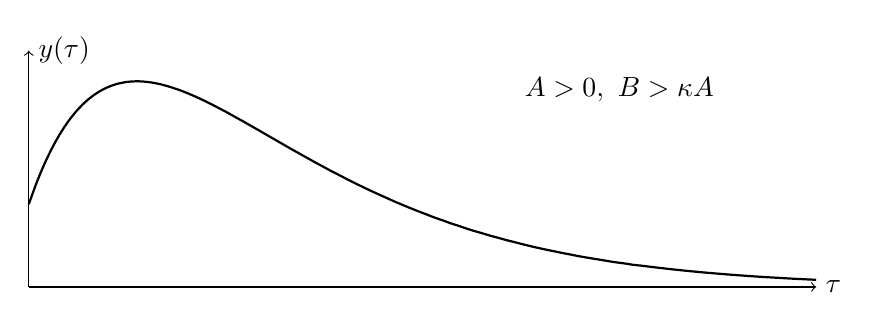
\begin{tikzpicture}
      \draw[->] (0, 0) -- (10, 0) node[right] {$\tau$};
      \draw[->] (0, 0) -- (0, 3) node[right] {$y(\tau)$};

      \node at (7.5, 2.5) {$A > 0,\ B > \kappa A$};

      \def\kconst{0.6}
      \draw[thick, domain=0:10, smooth, samples=100] plot (\x,{2.1 * exp(-\kconst*\x) * (0.5 + 1.7 * \x)});
    \end{tikzpicture}
    \end{center}
  \end{case}
  \begin{case}{Heavy Damping, $\kappa > 1$}
    $\lambda_1$ and $\lambda_2$ are real.
    WLOG, take $|\lambda_1| < |\lambda_2|$.
    \[
      \lambda_1 = \underbrace{-\kappa + \sqrt{\kappa^2 -1}}_{<0},\ \lambda_2 = \underbrace{-\kappa -\sqrt{\kappa^2 - 1}}_{<0}
    \]
    So the general solution is:
    \[
      y(\tau) = Ae^{-|\lambda_1|\tau} + Be^{-|\lambda_2|\tau}
    \]
    Since $|\lambda_1| < |\lambda_2|$, the first term dominates the long term behaviour provided $A \neq 0$.
    \begin{center}
    \begin{tikzpicture}
      \draw[->] (0, 0) -- (10, 0) node[right] {$\tau$};
      \draw[->] (0, -2) -- (0, 2.5) node[right] {$y(\tau)$};

      \def\kconst{1.5}
      \pgfmathsetmacro{\lone}{-\kconst + sqrt(\kconst^2 - 1)}
      \pgfmathsetmacro{\ltwo}{-\kconst - sqrt(\kconst^2 - 1)}
      \def\aconst{2.1}
      \def\bconst{-1.6}
      \node at (1.3, 2.0) {$Ae^{-|\lambda_1| \tau}$};
      \node at (1.2, -1) {$Be^{-|\lambda_2| \tau}$};
      \node at (4.5, 0.8) {$y(\tau)$};

      \draw[gray!70, dashed, domain=0:10, smooth, samples=100] plot (\x,{\aconst * exp(\lone*\x)});
      \draw[gray!70, dashed, domain=0:10, smooth, samples=100] plot (\x,{\bconst * exp(\ltwo*\x)});
      \draw[thick, domain=0:10, smooth, samples=100] plot (\x,{\aconst * exp(\lone*\x) + \bconst * exp(\ltwo * \x)});
    \end{tikzpicture}
    \end{center}
    As you can see, the initial behaviour of the solution is similar to that of $Be^{-|\lambda_2|\tau}$ but eventually the $Ae^{-|\lambda_1|\tau}$ dominates.
  \end{case}
\end{proofcases}
\begin{remark}[Note]
  In all three cases, the free/unforced response decays eventually towards 0.
\end{remark}
\subsection{Forced Response}
Initially, the solution will be similar to just C.F. + P.I, this is the \textit{transient response}.
But as time progresses, the system settles down to a specific particular integral, the \textit{steady state response}, for any choice of initial conditions.
\begin{example}
  Consider the ODE.
  Note that we are now just using normal $t$ instead of $\tau$.
  \[
    \ddot{y} + \mu \dot{y} + \omega^{2}_{0}y = \frac{F_0}{m}\sin \omega t \quad \mu = \frac{b}{m},\ \kappa = \frac{\mu}{2\omega_0}
  \]
  Assuming light damping ($\mu < 2 \omega_0$).
  So the complimentary function is:
  \[
    y_c = e^{-\frac{\mu t}{2}}(A\sin\omega_{\text{free}}t + B\cos\omega_{\text{free}}t) \quad \omega_{\text{free}} = \sqrt{\omega^{2}_{0} - \mu^2/4}
  \]
  Try a particular integral of the form:
  \[
    y_p(t) = \frac{F_0}{m}(C\sin\omega t+ D\cos \omega t)
  \]
  Substituting into the DE:
  \[
    \sin \omega t(-C\omega^2-D\mu\omega + \omega^{2}_{0}C) + \cos \omega t(-D\omega^2 + C\mu\omega + \omega^{2}_{0}D) = \sin \omega t
  \]
  Comparing coefficients of $\sin$ and $\cos$ yields:
  \[
    D(\omega^{2}_{0} - \omega^2) = -C\mu\omega,\ C(\omega^{2}_{0} - \omega^2) = 1 + D\mu\omega
  \]
  We can then eliminate $C$:
  \[
    -\frac{D(\omega^{2}_{0} - \omega^2)^2}{\mu \omega} = 1 + D\mu\omega \implies D=\frac{-\mu\omega}{(\omega^{2}_{0}-\omega^2)^2 + \mu^2\omega^2}
  \]
  and therefore:
  \[
    C = \frac{\omega^{2}_{0} - \omega^2}{(\omega^{2}_{0} - \omega^2)^2 + \mu^2\omega^2}
  \]
  Note that even if the driving has $\omega = \omega_0$, we do not end up with resonance issues because of the damping.
  If $\mu = 0$, then this would not be the case.

  Finally we can write $y_p$ as:
  \[
    y_p(t) = \frac{F_0/m}{(\omega^{2}_{0} - \omega^2)^2 +\mu^2\omega^2}[(\omega^{2}_{0} - \omega^2)\sin\omega t - \mu \omega \cos \omega t]
  \]
  If we then plot $y(t) = y_c + y_p$ together with $y_c$ and $y_p$, we see that the solution is originally influenced by both $y_c$ and $y_p$.
  This is the \textit{transient response}.
  Then as $t$ increases, $y_c$ decays so the solution approaches $y_p$.
  This is the \textit{steady-state response}.
  \begin{center}
  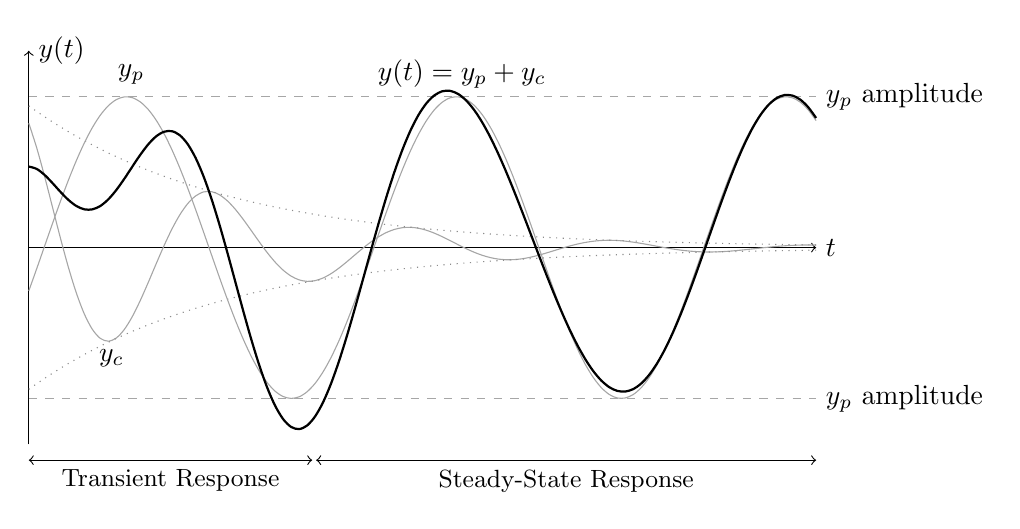
\begin{tikzpicture}
    \draw[->] (0, 0) -- (10, 0) node[right] {$t$};
    \draw[->] (0, -2.5) -- (0, 2.5) node[right] {$y(t)$};

    \def\omegazero{2.5}
    \def\omegaconst{1.5}
    \def\muconst{0.8}
    \def\fmconst{8}
    \def\cfamp{1.8}
    \def\cfphase{-0.5}
    \pgfmathsetmacro\omegafree{sqrt(\omegazero^2 - 0.25 * \muconst^2)}
    \pgfmathsetmacro\amplitude{(\fmconst)/(sqrt((\omegazero^2 - \omegaconst^2)^2 + \muconst^2 * \omegaconst^2))}
    \pgfmathsetmacro\tempconst{(\fmconst)/((\omegazero^2 - \omegaconst^2)^2 + \muconst^2 * \omegaconst^2)}

    \draw[gray!70, dashed] (0, \amplitude) -- (10, \amplitude);
    \draw[gray!70, dashed] (0, -\amplitude) -- (10, -\amplitude);
    \node[right] at (10, \amplitude) {$y_p$ amplitude};
    \node[right] at (10, -\amplitude) {$y_p$ amplitude};

    \draw[gray!70, domain=0:10, smooth, samples=100] plot (\x,{exp(-0.5 * \muconst * \x) * \cfamp * cos((\omegafree * \x - \cfphase) r)});
    \draw[gray!90, dotted, domain=0:10, smooth, samples=100] plot (\x,{exp(-0.5 * \muconst * \x) * \cfamp});
    \draw[gray!90, dotted, domain=0:10, smooth, samples=100] plot (\x,{-exp(-0.5 * \muconst * \x) * \cfamp});

    \draw[gray!70, domain=0:10, smooth, samples=100] plot (\x,{\tempconst * ((\omegazero^2 - \omegaconst^2) * sin(\omegaconst * \x r) - \muconst * \omegaconst * cos(\omegaconst * \x r))});

    \draw[thick, domain=0:10, smooth, samples=100] plot (\x,{\tempconst * ((\omegazero^2 - \omegaconst^2) * sin(\omegaconst * \x r) - \muconst * \omegaconst * cos(\omegaconst * \x r)) + exp(-0.5 * \muconst * \x) * \cfamp * cos((\omegafree * \x - \cfphase) r)});

    \node at (5.5, 2.2) {$y(t) = y_p + y_c$};
    \node at (1.3, 2.2) {$y_p$};
    \node at (1.05, -1.4) {$y_c$};

    \draw[<->] (0, -2.7) -- (3.6, -2.7) node[midway, below] {\small Transient Response};
    \draw[<->] (3.65, -2.7) -- (10, -2.7) node[midway, below] {\small Steady-State Response};
  \end{tikzpicture}
  \end{center}
\end{example}
\section{Impulses and Point Forces}
Consider a system that experiences a sudden force between time $t = T - \varepsilon$ and $t = T + \varepsilon$ for small $\varepsilon$:
\begin{center}
\begin{tikzpicture}[scale=1.3]
  \draw[->] (0, 0) -- (7, 0) node[right] {$t$};
  \draw[->] (0, 0) -- (0, 3) node[right] {$F(t)$};

  \node[below] at (2, 0) {$T - \varepsilon$};
  \node[below] at (3.5, 0) {$T$};
  \node[below] at (5, 0) {$T + \varepsilon$};

  \clip (0, 0) rectangle (8, 3);
  \draw[thick, domain=2:5, smooth, samples=100] plot (\x,{2.8*exp(-(\x - 3.5)^2) - 0.3});
\end{tikzpicture}
\end{center}
For example, when modelling striking a mass on a spring or a car going over a kerb.
\begin{example}
  \label{impulseExample}
  Recall from \cref{forcedODEs} the ODE that models a damped forced oscillator:
  \[
    m\ddot{y} + b\dot{y} + ky = F(t)
  \]
  It is mathematically convenient to consider the limit of a sudden impulse as $\varepsilon \to 0$.

  We can integrate the ODE from $T - \varepsilon$ to $T + \varepsilon$ and take then limit as $\varepsilon \to 0$:
  \[
    \lim_{\varepsilon \to 0^{+}} \left(m \eval{\dot{y}}{T - \varepsilon}{T + \varepsilon} + \underbrace{b \eval{y}{T - \varepsilon}{T+\varepsilon}}_{0 \text{ if $y$ continuous}} + \underbrace{k \int_{T-\varepsilon}^{T+\varepsilon} y \d{t}}_{0 \text{ if $y$ finite}}\right) = \underbrace{\lim_{\varepsilon \to 0^{+}} \int_{T-\varepsilon}^{T+\varepsilon} F(t) \d{t}}_{I\text{, Impulse}}
  \]
  We see that, if $y$ is finite and continuous, as $\varepsilon \to 0^{+}$, the only term that survives is the first term:
  \[
    \lim_{\varepsilon \to 0^{+}} \left(m \eval{\dot{y}}{T-\varepsilon}{T+\varepsilon}\right) =I
  \]
  So the velocity, $\dot{y}$, is discontinuous at $t = T$.
  As $\varepsilon \to 0$, only the impulse $I$ matters for subsequent motion.

  \begin{center}
  \begin{tikzpicture}
    \draw[->] (0, 0) node[left] {0} -- (10, 0) node[right] {$t$};
    \draw[->] (0, -2) -- (0, 2) node[right] {$y$};

    \def\kconst{0.2}
    \def\xoffset{4}
    \draw[thick, domain=2.25:10, smooth, samples=100] plot (\x,{2.1 * exp(-\kconst*(\x-\xoffset)) * (-0.1138 * sin((\x-\xoffset) * sqrt(1 - \kconst^2) r) + 0.8 * cos((\x - \xoffset)* sqrt(1 - \kconst^2)r))});

    \draw[thick] (0, 0) -- (2.26, 0) node[below] {$T$};
  \end{tikzpicture}
  \end{center}
\end{example}
\subsection{Dirac Delta Function}
The Dirac delta function formalises the concept of an impulsive force.
Consider the family of functions $D(t; \varepsilon)$ such that:
\[
  \lim_{\varepsilon \to 0} D(t; \varepsilon) = 0\ \forall t\neq0 \text{ and } \int_{-\infty}^{\infty} D(t; \varepsilon) \d{t} = 1
\]
The impulsive force we considered earlier in \cref{impulseExample} is then:
\[
  F(t) = ID(t - T; \varepsilon)
\]

One example of such a $D(t; \varepsilon)$ is:
\[
  D(t;\varepsilon) = \frac{e^{-t^2/\varepsilon^2}}{\varepsilon\sqrt{\pi}}
\]
For smaller $\varepsilon$, the distribution is more concentrated at 0, whereas for larger $\varepsilon$ it is more spread out.
\begin{center}
\begin{tikzpicture}
  \draw[->] (-5, 0) -- (5, 0) node[right] {$t$};
  \draw[->] (0, 0) node[below] {0} -- (0, 4) node[right] {$D(t; \varepsilon)$};

  \foreach \econst in {0.2, 0.6, 1.2} {
    \draw[thick, domain=-5:5, smooth, samples=100] plot (\x,{exp(-(\x/\econst)^2)/(\econst * sqrt(pi))});
  }
\end{tikzpicture}
\end{center}
Note that the area under the curve is always 1 regardless of $\varepsilon$ (See Example Sheet 1, Q14).

This family of functions is not unique, but for any family that has these properties, the limit as $\varepsilon \to 0$ yields the Dirac delta function.
\begin{definition}[Dirac Delta Function]
  The \textit{Dirac delta function} is defined by:
  \[
    \delta(t) = \lim_{\varepsilon \to 0} D(t; \varepsilon)
  \]
\end{definition}
\begin{remark}[Note]
  This is technically a \textit{distribution} not a function and only ``makes sense'' when used inside of an integral.
\end{remark}
\subsubsection{Properties}
\begin{enumerate}
  \item $\delta(t) = 0\ \forall t\neq 0$
  \item $\int_{-\infty}^{\infty} \delta(t) \d{t} = 1$
  \item For all functions $g(t)$ that are continuous at $t = 0$:
    \begin{align*}
      \int_{-\infty}^{\infty} g(t)\delta(t) \d{t} &= \lim_{\varepsilon \to 0} \int_{-\infty}^{\infty} g(t)D(t; \varepsilon) \d{t} \\
                                                  &=g(0) \lim_{\varepsilon \to 0} \int_{-\infty}^{\infty} D(t; \varepsilon) \d{t} \\
                                                  &=g(0)
    \end{align*}
    This is known as the \textit{sampling property}.
\end{enumerate}
More generally, for a function $g(t)$ continuous at $t = t_0$:
\[
  \int_{a}^{b} g(t)\delta(t - t_0) \d{t} = \begin{cases}
  g(t_0) & \text{ if }  a < t_0 < b \\
  0 & \text{ if $t_0 < a$ or $t_0 > b$} \\
  \text{undefined} & \text{ if $t_0 = a$ or $t_0 = b$}
  \end{cases}
\]
where $b > a$.
\subsection{Delta Function Forcing}
\label{deltaForcing}
Consider a 2nd order linear ODE with non-constant coefficients and forcing term $\delta(t)$:
\[
  y'' + p(x)y' + q(x)y = \delta(x)
\]
where $p, q$ are assumed to be continuous and $y$ is continuous at $x = 0$.
For $x < 0$ and $x > 0$, we just have the homogeneous equation:
\[
  y'' + p(x)y' + q(x)y = 0
\]
But we have a discontinuity in $y'$ at $x = 0$.
Integrating from $-\varepsilon$ to $\varepsilon$ and then taking the limit as $\varepsilon \to 0^{+}$ yields:
\[
  \lim_{\varepsilon \to 0^{+}} (\eval{y'}{-\varepsilon}{\varepsilon}) + p(0) \underbrace{\lim_{\varepsilon \to 0^{+}} (\eval{y}{-\varepsilon}{\varepsilon})}_{0 \text{ if $y$ continuous}} + \underbrace{\lim_{\varepsilon \to 0^{+}} \left(\int_{-\varepsilon}^{\varepsilon} q(x)y \d{x}\right)}_{0 \text{ if $y$ finite}} = 1
\]
So we then have:
\[
  \lim_{\varepsilon \to 0^{+}} \eval{y'}{-\varepsilon}{\varepsilon} = 1
\]
This is known as the \textit{jump condition}.
\begin{remark}[Note]
  The continuity of $y$ at $x = 0$ is required otherwise $y'$ is undefined at $x = 0$.
  We would then have $y' \propto \delta(x)$ with $y''$ being even worse behaved so it would not be possible for it to be a solution to the DE.
  (Further discussion on this later)
\end{remark}
In general, the highest-order term in the ODE ``addresses'' the delta function forcing as all the lower order terms must be finite (else we would run into the issues described above) so will vanish in the limit.
\begin{example}
  Find $y(x)$ for $0 \leq x \leq \pi$, where:
  \[
    y'' - y = 3\delta\left(x - \frac{\pi}{2}\right)
  \]
  with $y(0) = 0$ and $y(\pi) = 0$.

  For $0 \leq x < \frac{\pi}{2}$, $y'' - y= 0$ so:
  \[
    y = \alpha e^{x} + \beta e^{-x}
  \]
  Applying $y(0) = 0$ we see that $\alpha = - \beta$ thus $y = A \sinh x$ for some constant $A$.

  For $\frac{\pi}{2} < x \leq \pi$, we have the same DE but a different boundary condition, $y(\pi) = 0$:
  \[
    \alpha e^{\pi} + \beta e^{-\pi} = 0 \implies \beta = - \alpha e^{2\pi}
  \]
  Therefore:
  \[
    y = \alpha(e^{x} - e^{2\pi - x}) = -\alpha e^{\pi}(e^{\pi - x} - e^{-(\pi - x)}) = C\sinh(\pi - x)
  \]
  for some constant $C$.

  For $y$ to be continuous at $\pi / 2$, we need to join the solutions at $x = \frac{\pi}{2}$.
  \[
    A\sinh(\pi/2) = C\sinh(\pi/2) \implies A = C
  \]

  Now applying the jump condition:
  \begin{align*}
    \lim_{\varepsilon \to 0^{+}} \eval{y'}{\pi/2 - \varepsilon}{\pi/2 + \varepsilon} &= 3 \\
    -A\cosh(\pi/2) - A\cosh(\pi/2) &= 3 \implies A  = C = -\frac{3}{2\cosh(\pi/2)}
  \end{align*}
  So the final solution is:
  \[
    y(x) = \begin{cases}
    -\frac{3\sinh(x)}{2\cosh(\pi/2)} & \text{ if } 0 \leq x \leq \frac{\pi}{2} \\
    -\frac{3\sinh(\pi - x)}{2\cosh(\pi/2)} & \text{ if } \frac{\pi}{2} \leq x \leq \pi
    \end{cases}
  \]

  From the plot, we can see that $y$ is continuous at $\pi/2$ but $y'$ is not.
  \begin{center}
  \begin{tikzpicture}[scale=1.5]
    \draw[->] (0, 0) node[left] {0} -- (7, 0) node[right] {$t$};
    \draw[->] (0, -3) -- (0, 0.5) node[right] {$y$};

    \draw[dashed] (pi, 0) node[above] {$\frac{\pi}{2}$} -- (pi, -2.6);
    \node[above] at (2*pi, 0) {$\pi$};

    \pgfmathsetmacro{\Aconst}{-(3 / 2)*cosh(pi/2) * 0.3}

    \draw[thick, domain=0:pi, smooth, samples=100] plot (\x,{\Aconst * sinh(\x * 0.5)});
    \draw[thick, domain=pi-0.001:2*pi, smooth, samples=100] plot (\x,{\Aconst * sinh(pi -\x * 0.5)});
  \end{tikzpicture}
  \end{center}
\end{example}
\subsection{Heaviside Step Function}
\begin{definition}[Heaviside Step Function]
  The \textit{Heaviside} step function is defined by:
  \[
    H(x) = \int_{-\infty}^{x} \delta(t) \d{r}
  \]
\end{definition}
From the properties of the Dirac delta, it follows that:
\[
  H(x) = \begin{cases}
  0 & \text{ if } x < 0 \\
  1 & \text{ if } x > 0 \\
  \text{undefined} & \text{ if } x = 0
  \end{cases}
\]
From the fundamental theorem of calculus (\cref{FTC}), we also see that $H'(x) = \delta(x)$.
This makes sense as it is constant everywhere apart from 0 where it suddenly jumps up to 1.
When plotted, $H(x)$ looks like a step:
\begin{center}
\begin{tikzpicture}[scale=1.3]
  \draw[->] (-4, 0) -- (4, 0) node[right] {$x$};
  \draw[->] (0, 0) node[below] {0} -- (0, 3) node[right] {$H(x)$};

  \draw[very thick] (-4, 0) -- (0, 0);
  \draw[very thick] (0, 2) node[left] {1} -- (4, 2);

  \filldraw[fill=white, draw=black] (0, 2) circle (1.3pt);
  \filldraw[fill=white, draw=black] (0, 0) circle (1.3pt);
\end{tikzpicture}
\end{center}
We can also define the ramp function:
\[
  r(x) = \int_{-\infty}^{x} H(x) \d{x} = \begin{cases}
  0 & \text{ if }x\leq0 \\
  x & \text{ if }x\geq 0
  \end{cases}
\]
\begin{center}
\begin{tikzpicture}[scale=1.3]
  \draw[->] (-4, 0) -- (4, 0) node[right] {$x$};
  \draw[->] (0, 0) node[below] {0} -- (0, 3) node[right] {$r(x)$};

  \draw[very thick] (-4, 0) -- (0.01, 0);
  \draw[very thick] (0, 0) -- (3, 3);
\end{tikzpicture}
\end{center}
\begin{remark}
  In general, functions get smoother as we integrate.
\end{remark}
\subsubsection{Forcing with $H(x)$}
We might have a forcing term involving $H(x)$, for example, when modelling turning on a switch within a circuit.

If we have the ODE:
\[
  y'' + p(x)y' + q(x)y = H(x)
\]
where it is assumed that $p(x)$ and $q(x)$ are continuous at $x = 0$.
We can then write:
\[
  y'' + p(x)y' + q(x)y = \begin{cases}
  0 & \text{ if }x < 0 \\
  1 & \text{ if }x > 0
  \end{cases}
\]
Similarly to in \cref{deltaForcing}, we can integrate from $-\varepsilon$ to $\varepsilon$ and take the limit as $\varepsilon \to 0$:
\[
  \lim_{\varepsilon \to 0^{+}} \left(\int_{-\varepsilon}^{\varepsilon} y'' + p(x)y' + q(x)y \d{x}\right) = \lim_{\varepsilon \to 0^{+}} \left(\eval{y'}{-\varepsilon}{\varepsilon}\right) = \underbrace{\lim_{\varepsilon \to 0^{+}} \int_{0}^{\varepsilon} 1 \d{x}}_{= 0}
\]
However, unlike with the delta function, the right hand side is 0 instead of 1.
So $y'$ is also continuous at $x = 0$.

If we evaluate the DE at $\varepsilon$ and $-\varepsilon$ and then take the difference:
\[
  \eval{y''}{-\varepsilon}{\varepsilon} + \eval{p(x)y'}{-\varepsilon}{\varepsilon} + \eval{q(x)y}{-\varepsilon}{\varepsilon} = \eval{H(x)}{-\varepsilon}{\varepsilon}
\]
Then, as $\varepsilon \to 0$, we get:
\[
  \lim_{\varepsilon \to 0^{+}} \left(\eval{y''}{-\varepsilon}{\varepsilon} + \underbrace{p(0)\eval{y'}{-\varepsilon}{\varepsilon}}_{\to 0} + \underbrace{q(0)\eval{y}{-\varepsilon}{\varepsilon}}_{\to 0}\right) = 1
\]
So if $y'' \sim H(x)$ around $x = 0$ and both $y$ and $y'$ are continuous at $x = 0$ then this is satisfied.

Therefore, the jump conditions for the Heaviside function are:
\[
  \lim_{\varepsilon \to 0^{+}} \eval{y'}{-\varepsilon}{\varepsilon} = 0 \text{ and }
  \lim_{\varepsilon \to 0^{+}} \eval{y}{-\varepsilon}{\varepsilon} = 0
\]
That is, we require that both $y'$ and $y$ are continuous at $x = 0$.

Typically, we are told that $y = 0$ for $x < 0$.
We then solve for $x > 0$ and get a solution with two arbitrary constants and determine these by matching $y$ and $y'$ at $x = 0$.
Sometimes we instead solve in $x > 0$ and $x < 0$ and then match at $x = 0$.
\subsection{General Method for Heaviside and Delta Forcing}
The highest order derivative ``inherits'' the discontinuity of the forcing term.
This is is because if a lower order derivative had such a discontinuity, any higher order derivatives would have a more extreme discontinuities as differentiating makes functions less smooth in general.
This would mean that the discontinuities on one side of the equation would be more extreme than in the forcing term, so it would not be possible for it to satisfy the DE.

For example in the ODE:
\[
  y'' + 3y' + 2y = \delta(x)
\]
we expect $y'' \sim \delta(x)$ around $x = 0$ and, since integrating makes functions more smooth in general, we expect $y' \sim H(x)$ around $x = 0$ and expect $y$ to be continuous at $x = 0$.
\[
  \delta(x) \xrightarrow{\text{Integrating}} H(x) \xrightarrow{\text{Integrating}} \text{continuous}
\]
However in the ODE:
\[
  y' + 2y = \delta(x)
\]
we expect $y' \sim \delta(x)$ and $y \sim H(x)$ around $x = 0$.

To derive the exact jump conditions try integrating over the discontinuity from $T - \varepsilon$ to $T + \varepsilon$ and then taking the limit as $\varepsilon \to 0^+$.
For Heaviside forcing, also try evaluating both sides of the DE between $T - \varepsilon$ and $T + \varepsilon$ and then taking the limit as $\varepsilon \to 0^+$.

Then solve the ODE in all cases of the forcing function, remembering to use different constants for each discontinuous piece.
Finally, apply boundary and jump conditions, verifying that the final solution has the expected discontinuities/is continuous.
\section{Higher Order Discrete Equations}
Consider a linear, discrete, 2nd order equation with constant coefficients:
\[
  ay_{n + 2} + by_{n + 1} + cy_n = f_n
\]
\begin{remark}[Note]
These equations might arise when discretising a second order ODE.
\[
  \at{\deriv[2]{y}{x}}{x_n} \approx \frac{\overbrace{y(x_n + h)}^{y_{n + 1}} + \overbrace{y(x_n - h)}^{y_{n - 1}} - 2\overbrace{y(x_n)}^{y_n}}{h^2}
\]
\end{remark}
We can solve such equations with similar methods to ODEs by finding a complimentary function and a particular integral/solution:
\[
  y_n = y^{(c)}_n + y^{(p)}_n
\]
\subsubsection{Complimentary Functions}
Complimentary functions, $y^{(c)}$ satisfy the homogeneous discrete equation:
\[
  ay^{(c)}_{n + 2} + by^{(c)}_{n + 1} + cy^{(c)}_n = 0
\]
If we try $y^{(c)}_n \propto k^{n}$:
\begin{align*}
  ak^{n + 2} + bk^{n + 1} + ck^{n} = 0 \\
  \implies ak^2 + bk + c = 0
\end{align*}
which has roots $k_1$ and $k_2$.
This is the characteristic equation.
We then have general complimentary function:
\[
  y^{(c)}_n  = \begin{cases}
  Ak^{n}_{1} + Bk^{n}_{2} & \text{ if }k_1 \neq k_2 \\
  Ak^{n}_{1} + Bnk^{n}_1 & \text{ if }k_1 = k_2
  \end{cases}
\]
This is similar to how $y_c = Ae^{\lambda x} + Bxe^{\lambda x}$ for degenerate second order ODEs.
\subsubsection{Particular Integrals}
Similarly to with second order ODEs, we can use the form of the forcing term $f_n$ to guess what type of particular integral might work.
Again, we can superpose terms if needed as the equation is linear.
\begin{center}
\begin{tabular}{c|c}
$f_n$ & $y^{(p)}_n$ \\
\hline
$k^{n}$ & $Ak^{n}$ if $k \neq k_1 \text{ or }k_2$ \\
$k^{n}_{1}$ & $Ank^{n}_{1}$ \\
$n^{p},\ p \in \Z_{\geq 0}$ & $An^{p} + Bn^{p - 1} + \cdots + Cn + D$
\end{tabular}
\end{center}
\begin{example}[Fibonacci Sequence]
  Consider the discrete equation $y_n = y_{n - 1} + y_{n - 2}$ for $n \geq 2$ with boundary conditions $y_0 = 1$ and $y_1 = 1$.

  We first write this in the standard form:
  \[
    y_{n + 2} - y_{n + 1} - y_{n} = 0
  \]
  This has characteristic equation:
  \[
    k^2 - k - 1 = 0 \implies k = \frac{1 \pm \sqrt{5}}{2}
  \]
  These roots are the \textit{golden ratios}, $\phi_1$ and $\phi_2$:
  \[
    \phi_1 = \frac{1 + \sqrt{5}}{2} \approx 1.618\ldots \text{ and } \phi_2 = \frac{1 - \sqrt{5}}{2} =-\frac{1}{\phi_1}
  \]
  The general solution is then:
  \[
    y_n = A\phi^{n}_{1} + B\phi^{n}_2
  \]
  We then find $A, B$ from boundary conditions.
  \begin{align*}
    y_0 = 1 &\implies A + B = 1 \\
    y_1  = 1 &\implies A\phi_1 + B\phi_2 = 1 \\
             &\implies \frac{A + B}{2} + \frac{\sqrt{5}}{2}(A - B) = 1 \\
             &\implies A - B = \frac{1}{\sqrt{5}} \\
             &\implies A = \frac{1}{2}(1 + \sqrt{5}) = \frac{\phi_1}{\sqrt{5}},\ B = \frac{1}{2}\left(1 - \frac{1}{\sqrt{5}}\right) = \frac{1}{\sqrt{5}\phi_1}
  \end{align*}
  So the solution is:
  \[
    y_n = \frac{1}{\sqrt{5}}(\phi^{n + 1}_1 - \phi^{n + 1}_2) = \frac{1}{\sqrt{5}}\left(\phi^{n + 1}_1 - \left(-\frac{1}{\phi_1}\right)^{n + 1}\right)
  \]
  Since $\phi_1 > 1$, $y_n \to \frac{\phi^{n + 1}_1}{\sqrt{5}}$ as $n \to \infty$ so:
  \[
    \lim_{n \to \infty} \frac{y_{n + 1}}{y_n} = \phi_1
  \]
\end{example}
\section{Series Solutions}
When we cannot find simple closed form solutions, series solutions may be useful.

Consider a general second order linear homogeneous ODE:
\[
  p(x)y'' + q(x)y' + r(x)y = 0
\]
Note that this is a slightly different, but equivalent, form of the general equation.
Using the above form will simplify matters later.

The feasibility of finding a series solution around $x = x_0$ depends on the nature of $p(x)$, $q(x)$ and $r(x)$ around $x_0$.
\subsection{Classification of Singular Points}
\begin{definition}[Ordinary and Singular Points]
  The point $x = x_0$ is an \textit{ordinary point} if $\frac{q(x)}{p(x)}$ and $\frac{r(x)}{p(x)}$ are analytic at $x_0$.

  Otherwise, $x_0$ is a \textit{singular point.}
\end{definition}
\begin{remark}[Note]
  For our purposes, analytic means that we require $\frac{p(x)}{q(x)}$ and $\frac{r(x)}{p(x)}$ have a Taylor series about $x = x_0$ which converge in a region around $x_0$.
\end{remark}
\begin{definition}[Regular and Irregular Singular Point]
  If $x_0$ is a singular point and $(x - x_0)\frac{q(x)}{p(x)}$, $(x - x_0)^2\frac{r(x)}{p(x)}$ are analytic, then $x_0$ is a \textit{regular singular point}.
  Otherwise, $x_0$ is an \textit{irregular singular point}
\end{definition}
\begin{example}
  Consider an equidimensional 2nd order ODE:
  \[
    \underbrace{ax^2}_{p(x)} y'' + \underbrace{bx}_{q(x)}y' + \underbrace{c}_{r(x)}y = 0
  \]
  \[
    \frac{q}{p} = \frac{b}{ax} \text{ and } \frac{r}{p} = \frac{c}{ax^2}
  \]
  Both $\frac{q}{p}$ and $\frac{r}{p}$ are undefined at $x = 0$ so $x = 0$ is a singular point.

  Furthermore:
  \[
    x \frac{q}{p} = \frac{b}{a} \text{ and } x^2\frac{r}{p} = \frac{c}{a}
  \]
  which are both constants so $x = 0$ is a regular singular point.
\end{example}
\begin{example}
  \label{pointClassificationEx}
  \[
    \underbrace{(1 - x^2)}_{p(x)}y'' \underbrace{- 2x}_{q(x)}y' + \underbrace{2}_{r(x)}y = 0
  \]
  \[
    \frac{q}{p} = -\frac{2x}{1-x^2} = \frac{2x}{(x - 1)(x + 1)}
  \]
  So $\lim_{x \to \pm 1} \frac{q}{p}$ diverges.
  \[
    \frac{r}{p} = -\frac{2}{(x - 1)(x + 1)}
  \]
  Similarly, $\lim_{x \to \pm 1} \frac{r}{p}$ diverges.

  We therefore cannot write down the Taylor series about $x = \pm 1$ in either of the above cases.
  So we have singular points at $x = \pm 1$.

  For $x = + 1$:
  \[
    (x - 1)\frac{q}{p} = \frac{2x}{x + 1}\text{ and }
    (x - 1)^2\frac{r}{p} = -\frac{2(x - 1)}{x + 1}
  \]
  Both of the above are well behaved at $x = 1$ so $x = +1$ is a \textit{regular singular point}.

  Similarly, for $x = -1$:
  \[
    (x + 1)\frac{q}{p} = \frac{2x}{x - 1}\text{ and }
    (x + 1)^2\frac{r}{p} = -\frac{2(x + 1)}{x - 1}
  \]
  Both of the above are well behaved at $x = -1$ so $x = -1$ is also a regular singular point.
\end{example}
\begin{example}
  \[
    \underbrace{(1 + \sqrt{x})}_{p(x)}y'' \underbrace{- 2x}_{q(x)}y' + \underbrace{2}_{r(x)}y = 0
  \]
  \[
    \frac{q}{p} = -\frac{2x}{1 + \sqrt{x}}
  \]
  Consider $x_0 = 0$, although $\frac{q}{p}$ is well behaved as $x \to 0$, if we try and find the Taylor series, we find that the second derivative of $\frac{q}{p}$ is undefined at $x = 0$.
  So $x = 0$ is a singular point.
  \[
    x \frac{q}{p} = -\frac{2x^2}{1 + \sqrt{x}}
  \]
  This also does not have a Taylor series about $x = 0$.
  So $x = 0$ is an irregular singular point.
\end{example}
\subsection{Method of Frobenius}
\begin{theorem}[Fuch's Theorem]
  \label{fuchTheorem}
  \begin{enumerate}
    \item
      If $x = x_0$ is an \textbf{ordinary point}, then there are two linearly independent solutions of the form:
      \[
        y = \sum_{n = 0}^{\infty} a_n (x - x_0)^{n}
      \]
      which are convergent in some neighbourhood of $x_0$.
      That is, the solutions have a Taylor series about $x_0$ convergent in some neighbourhood of $x_0$.
    \item
      If $x = x_0$ is a \textbf{regular singular point}, then there is at least one solution of the form:
      \[
        y = \sum_{n=0}^{\infty} a_n(x - x_0)^{n + \sigma} = (x - x_0)^{\sigma} \sum_{n=0}^{\infty} a_n(x - x_0)^{n}
      \]
      where $\sigma \in \C$ and $a_0 \neq 0$ (as if we had $a_0 = 0$, the sum would effectively start at $n = 1$ so we could re-index and $\sigma$ would not be unique).
      This is called a \textit{Frobenius series}.
  \end{enumerate}
\end{theorem}
\begin{remark}[Note]
  In the case of a \textbf{regular singular point}, there is no guarantee that we obtain two linearly independent solutions.

  The series solution method may fail completely for an \textbf{irregular singular point}.
\end{remark}
\begin{example}[Ordinary Point]
  Find series solutions about $x = 0$ of
  \[
    (1 - x^2)y'' - 2xy' + 2y = 0
  \]
  From \cref{pointClassificationEx}, we see that $x = 0$ is an ordinary point and so we expect to find two linearly independent series solutions.

  Try $y = \sum_{n=0}^{\infty} a_nx^{n}$.
  We then have:
  \[
    y' = \sum_{n = 1}^{\infty} na_nx^{n - 1} \text{ and }y'' = \sum_{n = 2}^{\infty} n(n-1)a_nx^{n - 2}
  \]
  For convenience, multiply the ODE by $x^2$.
  \[
    (1 - x^2)\cdot x^2y'' - 2x \cdot x^2 y' + 2x^2y = 0
  \]
  Now substituting in yields:
  \[
    \sum_{n = 2}^{\infty} a_n[(1 - x^2)n(n-1)]x^{n} - 2\sum_{n=1}^{\infty} a_n n x^{n + 2} + 2 \sum_{n = 0}^{\infty} a_n x^{n + 2} = 0 \\
  \]
  We can rewrite the first sum as:
  \begin{align*}
    \sum_{n = 2}^{\infty} a_n[(1 - x^2)n(n - 1)]x^{n} &= \sum_{n=2}^{\infty} a_n n(n-1)x^{n} - \sum_{n = 2}^{\infty} a_n n(n - 1)x^{n + 2} \\
                                                      &= \sum_{n = 2}^{\infty} a_n n(n - 1)x^{n} - \sum_{n = 4}^{\infty} a_{n - 2}(n - 2)(n - 3)x^{n} \text{ ($n \mapsto n - 2$)}\\
                                                      &=  \sum_{n = 2}^{\infty} a_n n(n - 1)x^{n} - \sum_{n = 2}^{\infty} a_{n - 2}(n - 2)(n - 3)x^{n}
  \end{align*}
  The second sum can also be rewritten as follows:
  \begin{align*}
    -2\sum_{n=1}^{\infty} a_n n x^{n + 2} &= -2 \sum_{n = 3}^{\infty} a_{n - 2}(n - 2)x^{n} \text{ ($n \mapsto n -2$)}\\
                                          &= -2 \sum_{n = 2}^{\infty} a_{n - 2}(n - 2)x^{n}
  \end{align*}
  Similarly, for the third sum, we can re-index $n \mapsto n - 2$
  \[
    2 \sum_{n=0}^{\infty} a_n x^{n + 2} = 2 \sum_{n=2}^{\infty} a_{n - 2}x^{n}
  \]
  The sums now all go from $n = 2 \to \infty$ and only contain $x^{n}$ so we can easily equate coefficients of $x^{n}$ for $n \geq 2$:
  \begin{align*}
    a_n n(n - 1)& - a_{n - 2}(n - 2)(n - 3) - 2 a_{n - 2}(n - 2) + 2a_{n - 2} = 0 \\
    \implies n(n - 1)a_n &= (n^2 - 5n + 6 + 2n - 4 - 2)a_{n - 2} \\
                &= n(n - 3)a_{n - 2} \\
    a_n &= \frac{n - 3}{n - 1}a_{n  - 2}
  \end{align*}
  \begin{remark}[Advice]
    Whilst this method is very explicit, it is quite slow and it is often considerably faster to try to directly find the coefficient of $x^{n}$ as in \cref{regSPEx}.
  \end{remark}
  So we have found a recurrence relation for $a_n$.
  Note that because $a_0$ and $a_1$ are not determined, they are arbitrary constants in the general solution.

  Consider first the odd terms of the sequence.
  Notice that:
  \[
    a_3 = \frac{3 - 3}{3 - 1} a_1 = 0
  \]
  So $a_3 = a_5 = a_7 = \cdots = 0$.
  Therefore, one solution is $y = a_1 x$.
  Note that this is an even function of $x$.

  Now considering the even terms of the sequence
  \[
    a_n = \frac{n - 3}{n - 1}a_{n - 2} = \left(\frac{\cancel{n - 3}}{n - 1}\right)\left(\frac{n - 5}{\cancel{n - 3}}\right)a_{n - 4} = \cdots = - \frac{1}{n - 1}a_0
  \]
  Therefore, a second solution is:
  \[
    y = a_0 \left(1 - x^2 - \frac{x^4}{3} - \frac{x^{6}}{5} - \cdots\right)
  \]
  which is an even function of $x$, so we have separated the solution into an even and an odd component.

  Note that:
  \begin{align*}
    \ln (1 \pm x) &= \pm x - \frac{x^2}{2} \pm \frac{x^3}{3} - \frac{x^4}{4} \pm \frac{x^5}{5} + \cdots \\
    x\ln(1 \pm x) &= \pm x^2 - \frac{x^3}{2} \pm \frac{x^4}{3} - \frac{x^5}{4} \pm \frac{x^6}{5} + \cdots \\
    \implies x(\ln(1 + x) - \ln(1 - x)) &= 2x^2 + \frac{2x^4}{3} + \frac{2x^6}{5} + \cdots
  \end{align*}
  Therefore
  \begin{align*}
    y &= a_0 \left[1 - \frac{1}{2}(x\ln(1 + x) - x\ln(1 - x))\right] \\
      &= a_0 \left[1 - \frac{x}{2}\ln\left(\frac{1 + x}{1 - x}\right)\right]
  \end{align*}
  Alternatively, we could also notice that:
  \begin{align*}
    x^2 + \frac{x^4}{3} + \frac{x^{6}}{5} + \cdots &= x\left[x + \frac{x^{3}}{3} + \frac{x^{5}}{5} + \cdots \right] \\
                                                 &= x\left[\int (1 + x^2 + x^{4} + \cdots) \d{x}\right] \\
                                                 &= x\left[\int \frac{1}{1 - x^2} \d{x}\right] \\
                                                 &= x\artanh(x)
  \end{align*}
  In this example, we are able to write the general solution in closed form:
  \[
    y = a_1 x + a_0 \left[1 - \frac{x}{2}\ln\left(\frac{1 + x}{1 - x}\right)\right]
  \]
  Note the divergent behaviour near the singular points $x = \pm 1$.
\end{example}
\begin{example}[Regular Singular Point]
  \label{regSPEx}
  \[
    4xy'' + 2(1 - x^2)y' - xy = 0
  \]
  Since $\frac{2(1-x^2)}{4x}$ is not analytic at $x = 0$ but $2(1-x^2)$ is analytic at $x = 0$, $x = 0$ is a regular singular point.

  For convenience, we start by multiplying the DE by $x$.
  \[
    4x^2y'' + 2(1 - x^2)xy' - x^2y = 0
  \]
  Try $y=\sum_{n=0}^{\infty} a_n x^{n + \sigma}$, where $a_0 \neq 0$.
  \[
    \sum_{n=0}^{\infty} a_nx^{n + \sigma}[4\left(n + \sigma\right)(n + \sigma - 1) + 2(1-x^2)(n + \sigma) - x^2] = 0
  \]
  We will look at the lowest power of $x$ to determine $\sigma$, the lowest power is $x^{\sigma}$ which only occurs when $n = 0$.
  Comparing coefficients, we get:
  \begin{align*}
    a_0[4\sigma(\sigma - 1) + 2\sigma] &= 0  \\
    2a_0\sigma(2\sigma - 1) &= 0
  \end{align*}
  This is called the \textit{indicial equation}.
  Since $a_0 \neq 0$, we have either $\sigma = 0$ or $\sigma = \frac{1}{2}$.

  The next lowest power of $x$ is $x^{\sigma + 1}$ which only occurs when $n = 1$:
  \begin{align*}
    a_1 [4(\sigma + 1)\sigma + 2(\sigma + 1)] &= 0 \\
    2a_1(\sigma + 1) (2\sigma  + 1) &= 0
  \end{align*}
  Since $\sigma = 0$ or $\sigma = \frac{1}{2}$, we must have $a_1 = 0$.

  Now consider $x^{n + \sigma}$ for $n \geq 2$.
  Because $n \geq 2$, we get contributions from $x^{n - 2 + \sigma} \cdot x^2$ so we could expect to see $a_{n-2}$:
  \begin{align*}
    a_n4(n + \sigma)(n + \sigma - 1) + 2a_n(n + \sigma) - 2a_{n - 2}(n + \sigma - 2)- a_{n - 2} &= 0 \\
    2(n + \sigma)(2n + 2\sigma - 1)a_n &= (2n + 2\sigma - 3)a_{n - 2}
  \end{align*}
  First, consider $\sigma = 0$:
  \begin{align*}
    2n(2n - 1)a_n &= (2n - 3)a_{n -2} \\
    a_n &= \frac{2n - 3}{2n(2n -1)}a_{n-2}
  \end{align*}
  which us a recurrence relation for $a_n$.
  For the odd terms, we have $a_1 = 0$ so $a_3 = a_5 = a_7 = \cdots = 0$.
  For the even terms:
  \[
    a_2 = \frac{1}{4 \cdot 3}a_0,\ a_4 = \frac{5}{8 \cdot 7}a_2 = \frac{5 \cdot 1}{8 \cdot 7 \cdot 4 \cdot 3}a_0
  \]
  Therefore:
  \[
    y_1 = a_0\left[1 + \frac{x^2}{4\cdot3} + \frac{5x^4}{8\cdot 7 \cdot 4 \cdot 3} + \cdots\right]
  \]
  which is just a Taylor series.

  Now considering $\sigma = \frac{1}{2}$:
  \begin{align*}
    2\left(n + \frac{1}{2}\right)(2n + 1 - 1)a_n &= (2n + 1 - 3)a_{n -2} \\
    2n(2n + 1)a_n &= 2(n-1)a_{n-2}\\
    a_n &= \frac{n - 1}{n(2n  + 1)}a_0
  \end{align*}
  For the odd terms, we again have $a_1 = a_3 = a_5 = a_7 = \cdots = 0$.
  For the even terms:
  \[
    a_2 = \frac{1}{2 \cdot 5}a_0,\ a_4 = \frac{3}{4 \cdot 9}x_2 = \frac{3 \cdot 1}{4 \cdot 9 \cdot 2 \cdot 5}a_0, \ldots
  \]
  Therefore:
  \[
    y_2 = b_0x^{\frac{1}{2}}\left[1 + \frac{x^2}{2 \cdot 5} + \frac{3x^4}{4 \cdot 9 \cdot 2 \cdot 5} + \cdots\right]
  \]
  We relabeled the constant to $b_0$ as it does not have to be the same constant as in $y_1$ as we expect to have two arbitrary constants in the final solution.
  Note that this is an example of a Frobenius series.
\end{example}
\begin{remark}[Note]
  In this example, we were able to find two linearly independent solutions but we know from \cref{fuchTheorem} that this is not generally the case.
\end{remark}
\subsection{Second Solutions}
We are guaranteed to get one series solution about a regular singular point, but whether we get a second linearly independent such solution depends on the roots of the \textit{indicial equation}, say $\sigma_1$ and $\sigma_2$.
\begin{proofcases}
  \begin{case}{$\sigma_2 - \sigma_1$ \textbf{not} an integer}
    In this case, we get two linearly independent series solutions:
    \begin{align*}
      y_1 &= (x - x_0)^{\sigma_1}\sum_{n=0}^{\infty} a_n (x - x_0)^{n} \\
      y_2 &= (x - x_0)^{\sigma_2}\sum_{n=0}^{\infty} b_n (x - x_0)^{n}
    \end{align*}
    Note that if $\Re(\sigma_1) < \Re(\sigma_2)$ then $y_1$ will dominate as $x$ gets close to $x_0$.
  \end{case}
  \begin{case}{$\sigma_2 - \sigma_1$ is a \textbf{non-zero} integer}
    In this case, we get one series solution involving the larger root, say $\sigma_2 > \sigma_1$.
    \[
      y_1 = (x - x_0)^{\sigma_2}\sum_{n=0}^{\infty} a_n (x - x_0)^{n}
    \]
    The second solution has the form:
    \[
      y_2 = (x - x_0)^{\sigma_1}\sum_{n=0}^{\infty} b_n(x - x_0)^{n} + Cy_1(x)\ln(x - x_0)
    \]
    where $C$ is a constant that may or may not be zero.
    $C$ is determined in terms of $a_0$ and $b_0$, so we will have two arbitrary constants, as required.
  \end{case}
  \begin{case}{$\sigma_2 = \sigma_1 = \sigma$ -- Degenerate case}
    This is the similar to the second case, but we require $C \neq 0$ so that the two solutions are linearly independent.
  \end{case}
\end{proofcases}
\begin{example}[Case 2]
  \[
    x^2y'' - xy = 0
  \]
  Since $-\frac{1}{x}$ is not analytic at $x = 0$ but $-x$ is analytic at $x = 0$, $x = 0$ is a regular singular point.

  Try $y = \sum_{n=0}^{\infty} a_nx^{n + \sigma}$, where $a_0 \neq 0$.
  \[
    \sum_{n=0}^{\infty} \left[a_n(n + \sigma)(n + \sigma - 1)x^{n + \sigma} - a_nx^{n + \sigma + 1}\right] = 0
  \]
  In this case, the lowest power of $x$ is $x^{\sigma}$ which is only obtained when $n = 0$:
  \[
    a_0\sigma(\sigma -  1) = 0
  \]
  So $\sigma_1 = 0$ and $\sigma_2 = 1$.
  $\sigma_2 - \sigma_1 = 1$ which is a non-zero integer so we are indeed in case 2.

  For $n \geq 1$, since we can obtain $x^{n + \sigma}$ from $x^{n - 1 + \sigma + 1}$, we should expect to see $a_{n- 1}$:
  \[
    a_n (n + \sigma)(n + \sigma - 1) - a_{n - 1} = 0
  \]

  Starting with $\sigma_2 = 1$:
  \[
    a_n = \frac{a_{n - 1}}{n(n + 1)} \implies a_n = \frac{a_0}{n!(n + 1)!}
  \]
  Therefore:
  \[
    y_1 = a_0 x \left[1 + \frac{x}{2} + \frac{x^2}{12} + \frac{x^3}{144} + \cdots\right]
  \]

  Now with $\sigma_1 = 0$ we have:
  \[
    a_n n(n - 1) = a_{n - 1}
  \]
  But when $n = 1$, we have $a_0 = 0$ which is a contradiction.
  So as expected, we cant find another series solution like we did previously.

  At this point, to obtain a second linearly independent solution, we can either try a solution of the form:
  \[
    y_2 = \sum_{n=0}^{\infty} b_n x^{n} + Cy_1(x)\ln x
  \]
  or use a different method, such as reduction of order (see \cref{reductionOrder}).

  \nonexaminable
  To proceed using a series solution method, we can determine $\{b_n\}$ and $C$ by direct substitution into the ODE.

  We have:
  \begin{align*}
    xy_2 &= Cy_1 x\ln x + \sum_{n=0}^{\infty} b_n x^{n + 1} \\
    x^2y_2'' &= C(y_1'' x^2 \ln x + 2xy_1' - y_1) + \sum_{n=0}^{\infty} b_nn(n-1)x^{n}
  \end{align*}
  Thus:
  \begin{align*}
    x^2y_2'' - xy_2 &= C(\ln x (\overbrace{x^2 y_1'' -y_1x}^{=0}) + 2xy_1' - y_1) + \sum_{n=0}^{\infty} b_n[n(n-1)x^{n} - x^{n + 1}] \\
                    &= 2Cxy_1' - Cy_1 + \sum_{n=0}^{\infty} b_n[n(n-1)x^{n} - x^{n + 1}]
  \end{align*}
  So we require:
  \[
    2Cxy_1' - Cy_1 + \sum_{n=0}^{\infty} b_n[n(n-1)x^{n} - x^{n + 1}] = 0
  \]
  for $y_2$ to be a solution.
  From the series for $y_1$, we see that:
  \begin{align*}
    y_1 &= \sum_{n=0}^{\infty} a_n x^{n + 1} \text{ (as $\sigma_2 = 1$)} \\
    xy_1' &= \sum_{n=0}^{\infty} a_n(n + 1)x^{n + 1}
  \end{align*}
  So we require:
  \[
    C\sum_{n=0}^{\infty} a_n (2n + 1)x^{n + 1} + \sum_{n=0}^{\infty} b_n[n(n-1)x^{n} - x^{n + 1}] = 0
  \]
  The $x^{0}$ term vanishes but for $x^{n}$ with $n \geq 1$ we need:
  \[
    Ca_{n - 1}(2n - 1) + n(n - 1)b_n - b_{n - 1} = 0
  \]
  When $n = 1$, this gives $Ca_0 = b_0$ so $C = \frac{b_0}{a_0}$.
  Substituting in the expression for $a_n$ yields:
  \[
    \frac{2n - 1}{n!(n - 1)!}b_0 - b_{n - 1} +  n(n - 1)b_n = 0
  \]
  In this recurrence, we can choose $b_0$ and $b_1$ arbitrarily to then determine $b_n$ for all $n$ from there.

  Note that if $b_0 = 0$, then $y_2$ reduces to a multiple of $y_1$ so would not be a second linearly independent solution.
  In the case of $b_1 = 0$ we have:
  \[
    b_2 = -\frac{3}{4},\ b_3 = -\frac{7}{36}, \ldots
  \]
  So $y_2$ is then:
  \[
    y_2 = \frac{b_0}{a_0} y_1(x)\ln x + b_0\left[1 - \frac{3x^2}{4} - \frac{7x^3}{36} + \cdots\right]
  \]
\end{example}
\end{document}
